\chapter{Towards the Systematisation of Glyph Design}
\label{chap:strategies}

\begin{chapquote}{V. Gordon Childe}{``The aim of science is surely to amass and systematize knowledge.''}
\end{chapquote}

Glyph design has up until now been a largely ad-hoc design process fuelled by the tasks a user wishes to perform, and executed by a designer based almost entirely on a sample of the raw data, some data fields, and intuition. 
Although this may work in simple cases, it can result in: 
\begin{enumerate}
\item data types mapped to incorrect visual channels; 
\item data values mapped to too many visual channels (\eg too much colour); 
\item important information being hidden due to details not being visible at a working resolution; and 
\item ultimately glyphs that cannot be easily interpreted by their target audience. 
\end{enumerate}

Recent works by Colin Ware \cite{ware13} have gone some way to help inform visualization designers on how the visual system works (cognitive science) and best practices. 
Such works have been created due to a lack of information in the visualization community about how best to create visualizations by taking advantage of the human visual system.
Through aggregating some of the psychology and neuroscience literature into a digestible form, our intention is to make it easier for designers to exploit such information to make their visualizations more effective.
%
%\begin{figure}[ht!]
%\centering
%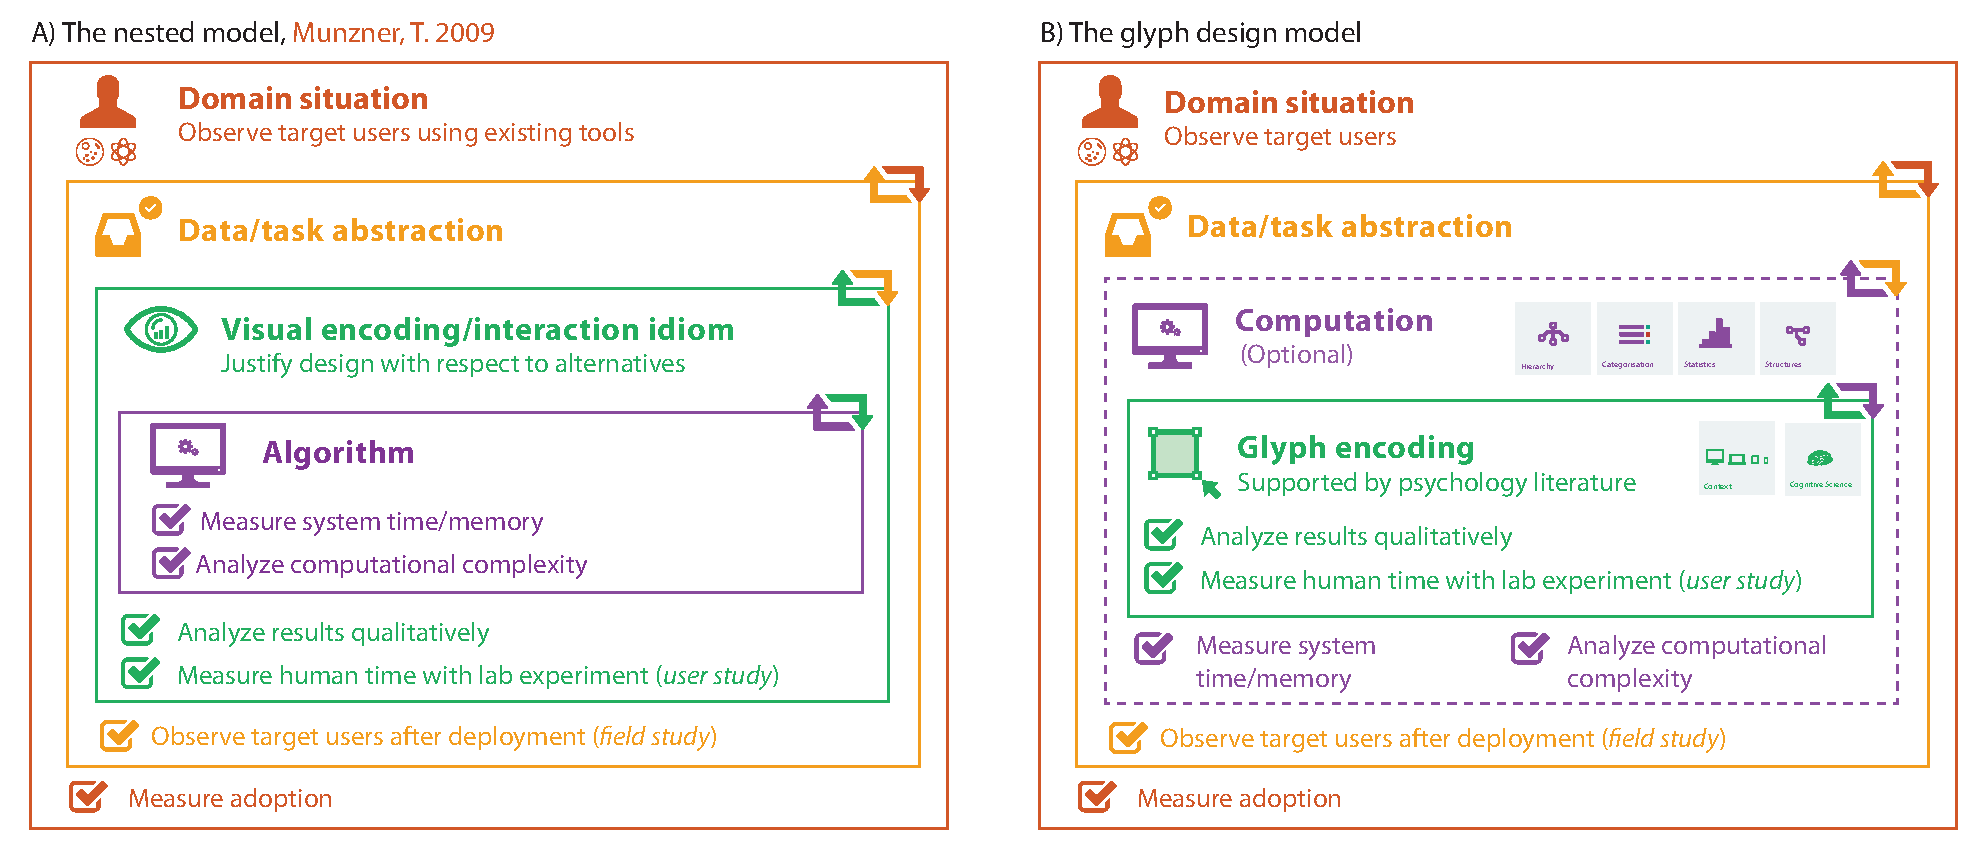
\includegraphics[width=\textwidth]{images/ch3/model}
%\caption{A) An overview of the ``nested model'' presented by Munzner \etal \cite{munzner2009nested}. B) A ``glyph design model'' inspired by the ``nested model''.}
%\label{fig:systematisation-models}
%\end{figure}

\begin{figure}[t!]
\centering
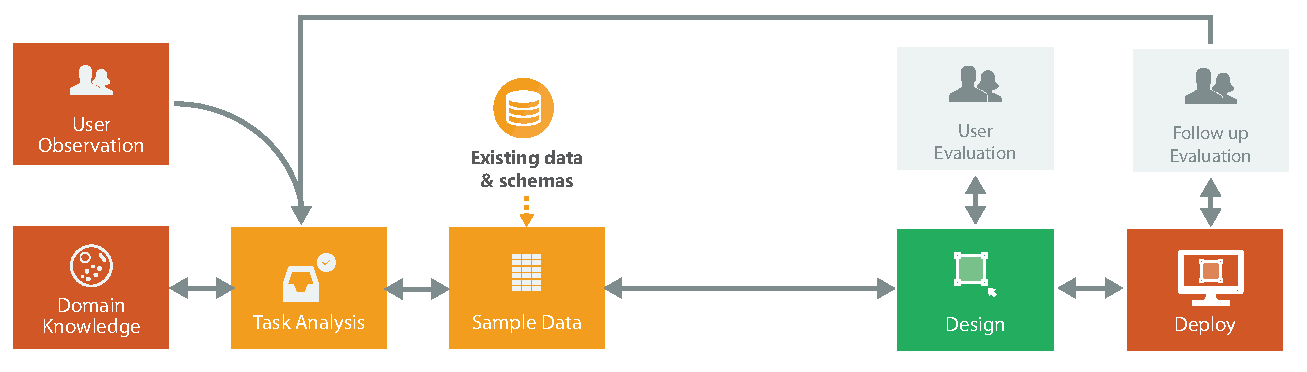
\includegraphics[width=\textwidth]{images/ch3/model_horizontal_simple}
\caption{A typical glyph design process modelled upon the ``nested model'' by Munzner \cite{munzner2009nested} where a designers instinct and iterations based on feedback from domain experts is core to the process.}
\label{fig:simple_process}
\end{figure}


Figure \ref{fig:simple_process} shows a typical representation of the glyph design process mapped to the components of the frequently followed ``nested model'' for visualization design by Munzner \cite{munzner2009nested}.
This model has the following components at its core:

\begin{itemize}
\item \textbf{User Observation} provides an opportunity to monitor users in their normal working environment.
Knowledge gained from this process can feed in to:
\begin{enumerate}
	\item \emph{task} definition through interviews and day to day observations of current working practices;
	\item \emph{design} processes via information about what a user is: willing to learn; willing to remember; and is able to remember. This ultimately affects the number of variables that can be encoded and how they are encoded. If a user has little time to remember glyphs, then they should be more accessible via increased use of metaphor for example; and 
	\item \emph{evaluation} to determine whether or not the solution meets user expectations and solves the problem the glyph was meant for.
\end{enumerate}

\item \textbf{Domain Knowledge} is of importance in any visualization since a good understanding of the domain will generally result in better visualizations that really solve the problems faced by the users.
Furthermore, domain knowledge carries additional importance in glyph-based visualization due to the common need for metaphor to support glyph learnability and memorability;

\item \textbf{Task Analysis} (or data/task abstraction in the ``nested model'') provides an indication of the types of visual queries that a user would like to make.
These tasks form the basis of data prioritisation.
For example, if a major task performed by a user was finding users of a particular age, making the age information more visually available is important;

\item \textbf{Sample Data} gives an indication of the data values (and ranges) to be encoded by the glyphs.
%These values can be processed by algorithms (see the \emph{computation} section) to find the most common values, the rarest values, and so forth depending on the visualization requirements.
A \emph{data representation schema} can provide additional information about the format of the sample data and the types of values  (\eg, categorical or quantitative) each field contains.
This in turn can be used in the design phase where design principles discussed below can be applied to ensure that appropriate visual channels are used for particular data values;

\item \textbf{Design} involves the selection of appropriate visual channels to represent each data variable to be encoded followed by the arrangement of those visual channels in 2D or 3D space;


\item \textbf{Evaluation} provides some level of validation that the glyph design is a success.
However, there are numerous ways in which a glyph may be evaluated.
They may be validated by reviewing the tasks defined earlier with users.
Glyphs could be evaluated in terms of their distinguishability, to ascertain whether or not users can detect differences between glyphs (if users cannot distinguish between glyphs, visual search will be impeded)?
If glyphs are providing an alternative to an existing visualization system, benchmarks on user accuracy and task speed can be made for comparison purposes.
If a glyph design does not perform effectively, there will be further iterations on the design to improve performance. 
When a design is approved, glyphs may be deployed in the day to day working environment of the domain experts.
Follow up studies can be conducted over time, and more iterations may be required.
\end{itemize}

Although this model represents the common visualization design practices, it does not offer direct solutions to help systematise glyph design.
Much of the details are still left up to individual designers to negotiate with domain experts.
In this way, the design process is referred to as \emph{ad hoc} (``for this'').
Due to a need for domain specific metaphor in glyph design, an \emph{ad omnia} (``for everything'') design process is unlikely to exist.
However, through incorporation of design principles, more objective decision making can be performed to control data to visual channel mappings for instance.
Additionally, computational techniques can present further opportunities to directly and indirectly (by proposing data features to be encoded) guide glyph design.

\begin{figure}[t!]
\centering
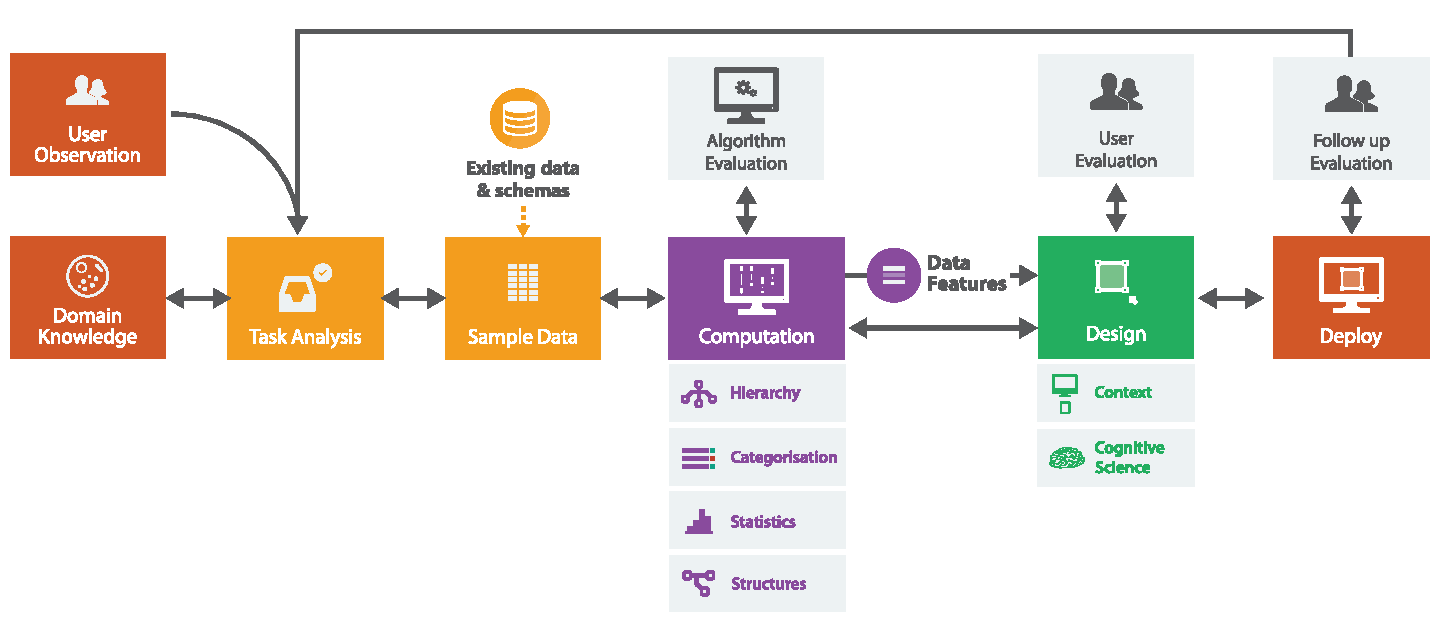
\includegraphics[width=\textwidth]{images/ch3/model_horizontal_new}
\caption{A more systematic approach to glyph design using computation to either directly inform the design step, or to provide data features to be used for glyph design. The design step is influenced by design principles and context.}
\label{fig:new_process}
\end{figure}

This chapter proposes an approach illustrated in Figure \ref{fig:new_process} for the systematic creation of glyphs.
Central to this approach is the addition of computational techniques to the model in Figure \ref{fig:simple_process}, and a more structured approach to the selection and arrangement of visual channels in the design step.
Our additions are there to reduce the reliance on subjectivity in the design process, however, staying true to the ``nested model'' \cite{munzner2009nested}, the importance of domain-expert interaction and evaluation is not downplayed.

The remainder of this chapter goes in to more detail on how these \emph{design} and \emph{computation} steps break down, and how individually and collectively they can contribute to more systematic and predictable glyph design.

\section{Design Principles}

\begin{figure}[t!]
\centering
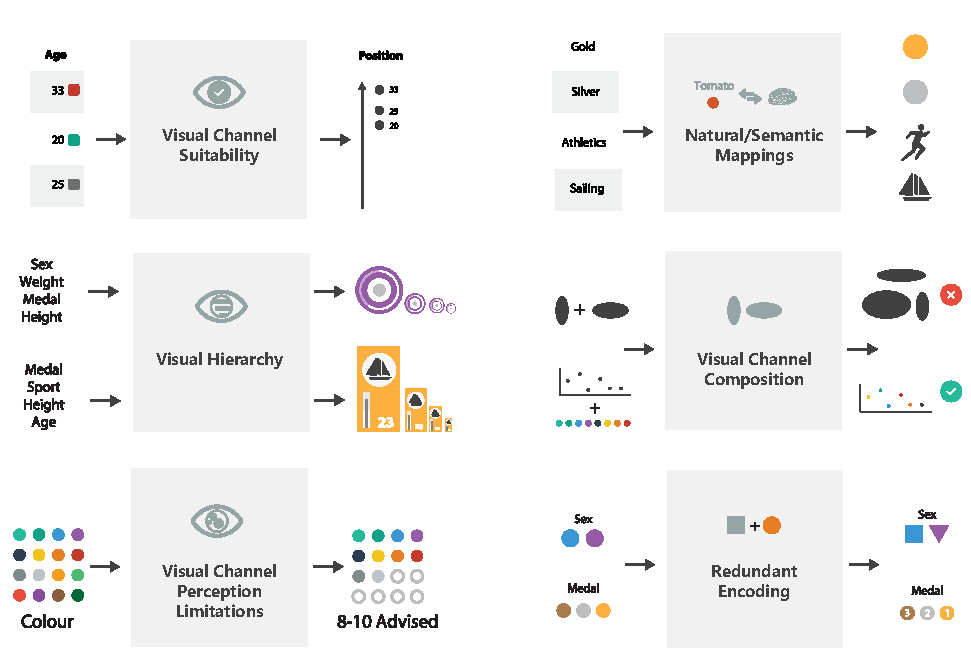
\includegraphics[width=\textwidth]{images/ch3/design_guidelines_2}
\caption{Design principles that can be followed to provide a more systematic approach to glyph design.}
\label{fig:strategies_design_guidelines}
\end{figure}

Ultimately, the goal of a systematic technique is to remove the level of randomness in some process.
For glyphs, the levels of randomness can be limited through integrating knowledge of how the visual system works in to the design process.
Core to such a process are a set of design principles based on research stated in Chapter \ref{chap:related_work} and illustrated in Figure \ref{fig:strategies_design_guidelines} consisting of:

\begin{enumerate}

\item \textbf{Visual channel suitability} in advises that data types within a glyph should be mapped to the correct visual channels.
This is based on work by Stevens \cite{stevens1975}, Bertin \cite{Bertin:1983:book}, Cleveland and McGill \cite{cleveland1984graphical}, Mackinlay \cite{mackinlay1986automating}, Heer and Bostock \cite{heer2010crowdsourcing};

\item \textbf{Natural mappings} suggests the use of semantically meaningful mappings of data to their natural visual counterparts where possible.
Using too many abstract colours or shapes for example would place a lot of cognitive load on a user to remember all mappings.
Make these colours or shape metaphoric however, and the glyph decoding process will be much easier, \eg, \textcolor{Red}{strawberry $\Leftrightarrow$ red}, \textcolor{Plum}{aubergine $\Leftrightarrow$ purple}, or \textcolor{Green}{money $\Leftrightarrow$ green} \cite{lin2013selecting}.
This principle is based work by Ware \cite{ware2010visual, ware13}, Borgo \etal \cite{Borgo12}, and Lin \etal \cite{lin2013selecting};

\item \textbf{Visual hierarchy} applies an organisation to the visual channels within a glyph given the importance of the data to some task.
This ensures that the most important classifiers of data are available even at the overview level of a visualization due to their visual prominence (visual hierarchy and global/local processing, and pre-attentive processing);

\item \textbf{Visual channel composition} suggests avoiding visual channels that are perceived holistically as opposed to separately.
The integrality or separability of a pair of visual channels is not a discrete decision.
While it is largely agreed that width and height are the most integral dimensions, while position and colour are the most separable, many other dimension lie on a continuum between fully integral and fully separable; 

\item \textbf{Visual channel perceptual limitations} provides guidance to avoid overuse of a visual channel such as colour whose perception degrades as the number of samples from each hue increases.
For example, distinguishing between four distinct colour hues is possible, but it is much harder to distinguish between sixteen distinct colours.
Colour maps like those provided in \emph{ColorBrewer} \cite{ColorBrewer} and \emph{Tableau} \cite{tableau_palettes} provide a good starting point for glyph designers; and

\item \textbf{Redundant encoding} suggests the use of multiple encodings for one data item so as to minimise the chance of error when reading glyphs in a display \cite{ware13}.
Redundant encoding may also speed up visual search.
For example, in Figure \ref{fig:strategies_design_guidelines} F, colour and shape are used to code gender.
Therefore, if the colour channel is impeded, shape can be used to distinguish between male and female glyphs.
\end{enumerate}

\section{Computation}

\begin{figure}[h!]
\centering
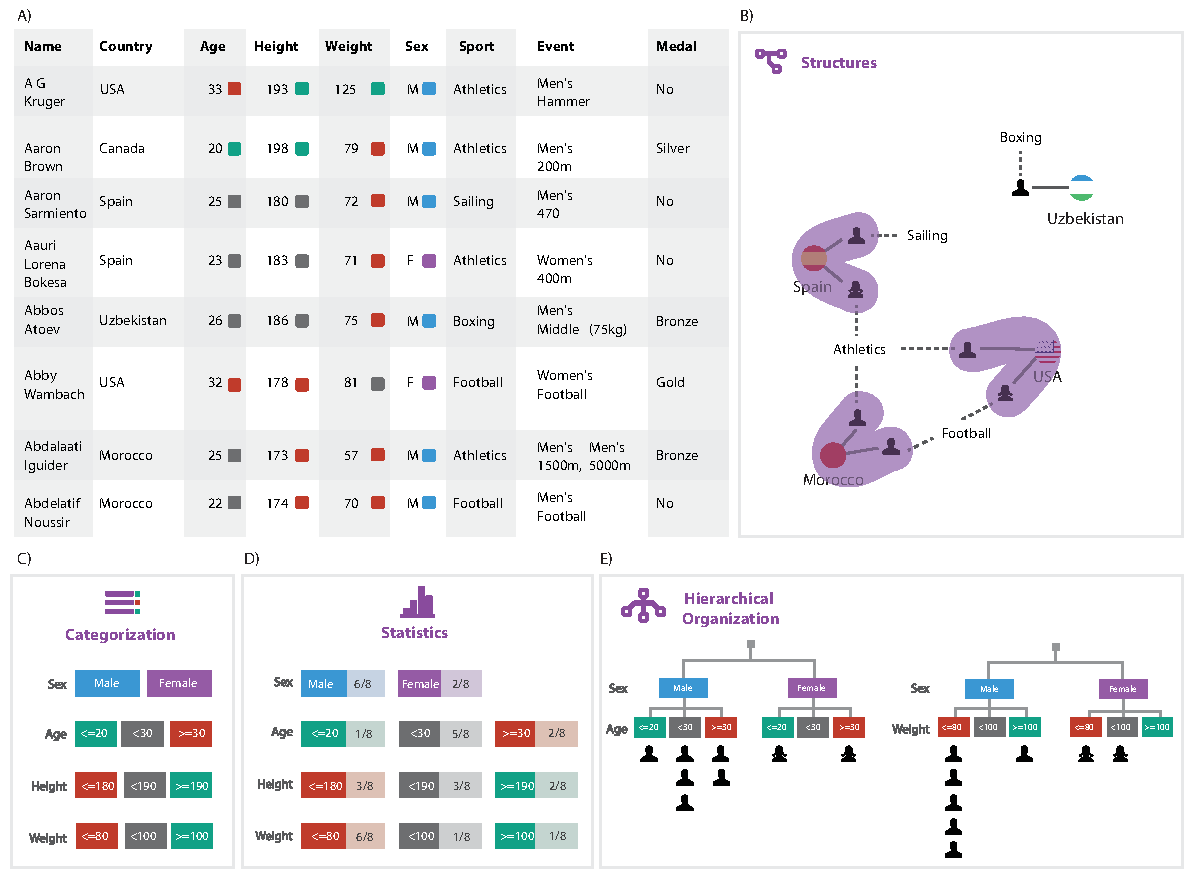
\includegraphics[width=\textwidth]{images/ch3/computation_benefits}
\caption{A) Table showing a subset of London 2012 Olympians with country, age, height, weight, sex, general sport, events, and if they won a medal.
B) By building a graph from the data from the table in A) certain structures can be mined in the data. Common structures in graphs or motifs could be a target for aggregation when the graph is very large.
C) We can create categories from the data that can be used directly to colour code ranges of values for instance.
D) Statistics can provide an indication of how balanced particular categories are, or what values are very common or very rare so that they may be highlighted or hidden depending on the user task.
E) Using categories from C) we can generate a tree/taxonomy that classifies the data in a structured way.
The choice of category will ultimately change the properties of the tree including how balanced it is (\eg, the tree on the left is more balanced than the one on the right since people are more evenly distributed at the leaf nodes).}
\label{fig:computational_benefits}
\end{figure}

Computation can be deployed to provide additional information about the data (derived data).
We have identified four techniques that can be applied either individually or combinatorially to help the glyph design process.
This influence may be direct, where the output of computation can be used to design glyphs.
Or it may be indirect, where computation identifies the features to be encoded using glyphs.
\begin{enumerate}

\item \textbf{Structure identification} (Figure \ref{fig:computational_benefits} B) generally refers to discovery of patterns in relational data, \eg, patterns in connectivity.
This information can be used to reduce complexity in network visualizations by removing common or uninteresting patterns, leaving behind the more important signals.
Figure \ref{fig:structure_compress_glyph} shows an example where we wish to find the common elements (motifs) in a graph and substitute these motifs with less complex glyph representations. 
Simple motif finding can be accomplished using an algorithm such as FANMOD \cite{wernicke06}.
This finds similar topologies in a graph and counts their occurrence.
The most common motifs are then put forward to be substituted in a simplified graph.

\begin{figure}[h!]
\centering
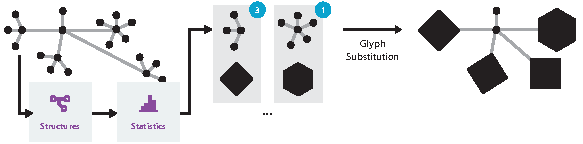
\includegraphics[width=\textwidth]{images/ch3/structure_compress_glyph}
\caption{Graph-based compression can make use of glyphs through the substitution of common structures/pattern/motifs with glyph alternatives.
This can be used to greatly reduce graph complexity as by Dunne \etal \cite{dunnemotif2012}.}
\label{fig:structure_compress_glyph}
\end{figure}

\item \textbf{Categorizations} (Figure \ref{fig:computational_benefits} C) provide a way of splitting the data based on various categorisations.
For example, in Figure \ref{fig:computational_benefits} C, there are four classifications schemes for sex, age, height and weight.
Each of these schemes has a number of ``classes'', and the data is likely to be distributed differently across those different categories.
These schemes could be determined computationally using algorithms such as k-means \cite{macqueen1967} or hierarchical-based (\eg, \cite{Sibson01011973}) clustering.
However these approaches are often inaccurate and computationally expensive.
Another approach is to use a more supervised approach to clustering with the aid of computation, a large representative data set, and domain experts in the loop to ensure that categorisations are meaningful and not too granular.

Such categorisations, when computed can be used to group data records based on a range of values, rather than singletons.
For example, in Figure \ref{fig:computational_benefits} C athletes can be grouped by their age, height, or weight range.
What this means in terms of glyph design is that instead of representing every possible age, height, or weight, we can represent just three ranges showing the normal and two outlier ranges.
Going back to Chapter \ref{chap:related_work}, this has implications for improved visual search, since now to find a class of value, a user need only search for one of three values.
Comparing between three sizes, colours, or shapes is much easier than between ten or more.

\item \textbf{Statistics} (Figure \ref{fig:computational_benefits} D) is generally helpful since it can provide information about the distribution of data, this can feed in to the categorisation process for example.
Statistical processes can also help identify the common/rare data features to be encoded using glyphs to bring attention to such features in a visualization.

\begin{figure}[t!]
\centering
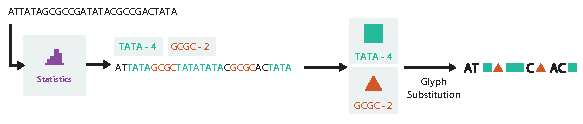
\includegraphics[width=\textwidth]{images/ch3/statistics_compression}
\caption{Text-based compression can use glyphs to replace common text with visual representations.
In this case, some common DNA motifs are replaced with coloured shapes.
Since reading text is a cognitively demanding process, showing structures of interest visually can speed up interpretation.
}
\label{fig:text_compress_glyph}
\end{figure}

For example, in Figure \ref{fig:text_compress_glyph} statistical processes are used to find the most common four letter sequences in a string representing a small region of DNA.
By finding the common elements and replacing them with coloured shapes, the \textcolor{Green}{TATA} and \textcolor{red}{GCGC} regions can be found more easily in the DNA sequence using glyphs rather than text.
This technique takes advantage of the supposed iconic memory identified by Sperling \cite{sperling60}.

\item \textbf{Hierarchical Organization} (Figure \ref{fig:computational_benefits} E) refers to the creation of a taxonomy, a tree representation that hierarchically defines the properties of items (leaf nodes) in the tree.
Maguire illustrated many examples of taxonomies in biology and visualization \cite{maguire12} including the tree of life in biology that categorises all species by their Kingdom --> Phylum --> Class --> Order --> Family --> Genus --> Species. 
For glyph design this hierarchical organisation can be used to structure how a glyph is arranged.
Imposing an order to the design should facilitate better learnability and memorability of the resulting glyphs since the formation of each glyph should follow a rule.

\begin{figure}[h!]
\centering
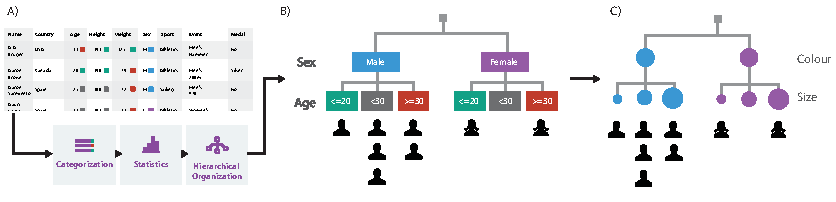
\includegraphics[width=\textwidth]{images/ch3/table_tax_glyph}
\caption{A) Starting with our table of Olympians, categorize the data, perform the statistical analysis, and generate the hierarchical organization.
B) The result of the hierarchical organization process is a taxonomic tree that represents the original data in a structured way.
C) From the hierarchical results, a glyph can be designed by assigning a visual channel to each level in the taxonomic tree where the visual channel assigned is decided by data type, and the ``strength'' of the visual channel.}
\label{fig:taxonomic_glyph_design}
\end{figure}

Figure \ref{fig:taxonomic_glyph_design} shows how one may traverse from a collection of records in a table to a taxonomic tree, then a glyph based representation of people within that tree by sex and age categories.

\end{enumerate}

\section{Summary}

So far, we have presented a hypothesis on how glyph design could be made better, and outlined a ``model'' in Figure \ref{fig:new_process} that could be followed to test this hypothesis.
The remainder of this thesis will apply this model to a number of scenarios and investigate how design principles and computation can contribute to a more systematic glyph design.

All further chapters apply different mixtures of design strategies by using flavours of the model defined here where computation and evaluation techniques in particular will vary.
Listed below is a summary of the work conducted in this thesis and the strategies used in relation to our systematic framework shown in Figure \ref{fig:strategies_examples}

\begin{figure}[b!]
\centering
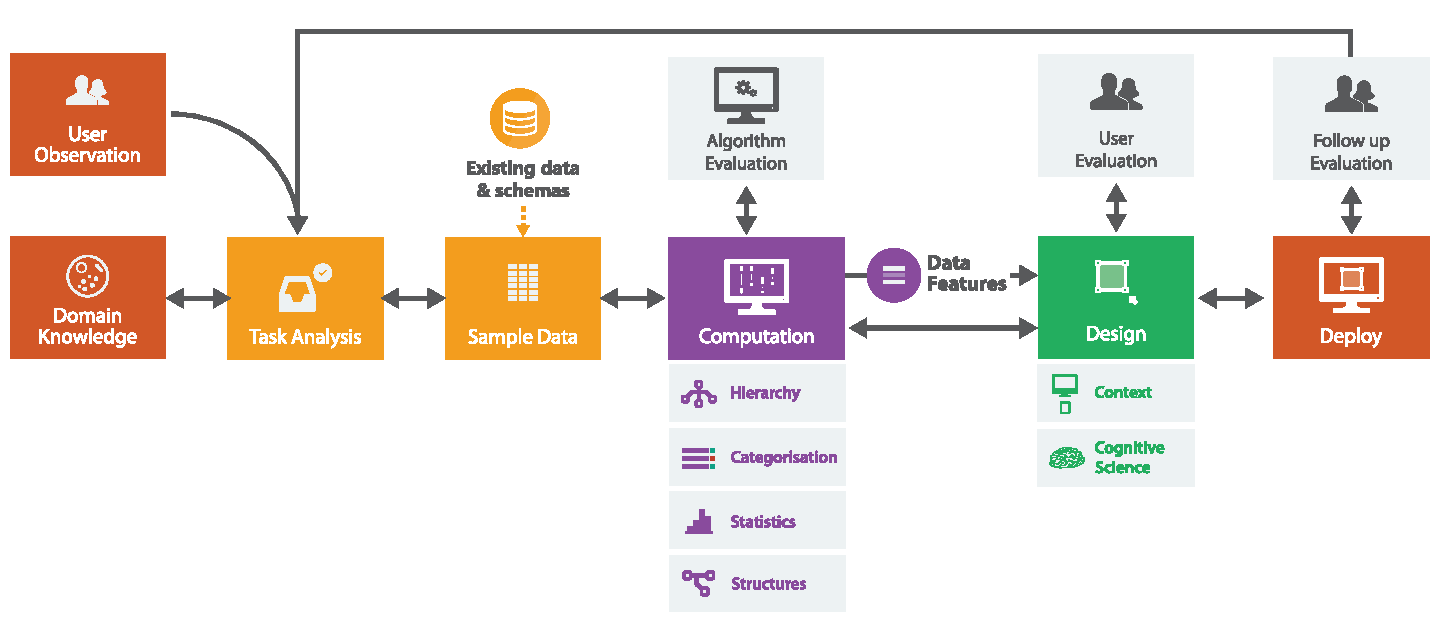
\includegraphics[width=\textwidth]{images/ch3/model_horizontal_new}
\caption{Our framework for more systematic glyph creation.}
\label{fig:strategies_examples}
\end{figure}


\begin{enumerate}

\item \textbf{Chapter \ref{chap:glyph-tax}}:
\begin{itemize}
\item \emph{Users:} Biologists (domain experts involved in work).
\item \emph{Sample Data:} ArrayExpress \cite{ArrayExpress::2012} repository with over 1.2 million individual experiments.
\item \emph{Computation:} Categorisation, statistical analysis, and hierarchical organisation of biological sample characteristics (\eg, organism, organism parts) and processes.
\item \emph{Design:} Uses the computationally generated taxonomy in combination with visual channel orderings and design principles.
\item \emph{Evaluation:} Domain expert evaluation (two biologists and trained data curators from the University of Oxford).
\item \emph{Deployment:} Used in a popular data annotation and curation tool called ISAcreator \cite{rocca-serra10}.
\end{itemize}

\item \textbf{Chapter \ref{chap:automacron}}:
\begin{itemize}
\item \emph{Users:} Biologists (domain experts involved in work).
\item \emph{Sample Data:} ArrayExpress \cite{ArrayExpress::2012} repository with over 1.2 million biological experiments.
\item \emph{Computation:} Structure analysis of biological workflow graphs from Chapter \ref{chap:glyph-tax}, and statistical analysis.
\item \emph{Design:} Uses the motif finding algorithm to automatically generate multi-resolution glyphs by following design principles.
\item \emph{Evaluation:} Motif finding algorithm performance comparison and domain expert evaluation (two biologists and trained data curators from the University of Oxford).
\item \emph{Deployment:} Available as a standalone tool for error detection tasks, and to build macro glyph libraries.
Also used in the ISAcreator \cite{rocca-serra10} tool to compress common patterns in biological workflows.
\end{itemize}

\item \textbf{Chapter \ref{chap:timeseries}}:
\begin{itemize}
\item \emph{Users:} Zoologists and statisticians (Oxford University), and analysts at an online betting company.
\item \emph{Sample Data:} Space shuttle and electrocardiogram data from Keogh \etal \cite{shuttle_data} .
\item \emph{Computation:} Statistical analysis to identify common time series patterns and count their occurrence.
\item \emph{Design:} Uses design principles to drive the glyph creation process.
\item \emph{Evaluation:} Baseline comparison with ground truth anomalies. Users from industry (online casino), and zoologists from the University of Oxford tested the interface and algorithm results.
\item \emph{Deployment:} General purpose web application.
\end{itemize}

\item \textbf{Chapter \ref{chap:processes}} introduces a number of additional examples showing how the systematicism introduced in this thesis can be applied to areas such as biological sequence analysis, poetry, and security analysis.
These examples also use different evaluation approaches, and the last example introduces a method to perform some quantitive evaluation on glyphs.
\begin{enumerate}
\item Biological sequence visualization:
\begin{itemize}
\item \emph{Users:} Biologists/Bioinformaticians.
\item \emph{Sample Data:} DNA sequences for the same region in 1809 bacteria.
\item \emph{Computation:} None.
\item \emph{Design:} design principles followed to drive the glyph creation process.
\item \emph{Evaluation:} A domain expert (Dr. Philippe Rocca-Serra, a biologist from the University of Oxford) was involved in the design process throughout, followed by an online user survey with forty-two biologists and bioinformaticians.
\item \emph{Deployment:} Open-source sequence logo library viewer for the web.
\end{itemize}

\item Poetry visualization:
\begin{enumerate}
\item \emph{Poetry glyph}:
\begin{itemize}
\item \emph{Users:} Humanities scholars (poets).
\item \emph{Sample Data:} Numerous poetry, English texts and scientific literature.
\item \emph{Computation:} None.
\item \emph{Design:} design principles followed to drive the glyph creation process.
\item \emph{Evaluation:} Two poets (from the University of Utah), and a language scholar (from the University of Oxford) were involved in the design process.
The same experts evaluated the resulting software tool.
\item \emph{Deployment:} An online tool called PoemViewer \cite{CGF:Abd2013a}.
\end{itemize}
\item \emph{Macro glyph}:
\begin{itemize}
\item \emph{Users:} Humanities scholars (poets).
\item \emph{Sample Data:} Numerous poetry, English texts and scientific literature.
\item \emph{Computation:} Statistical and structural analysis.
\item \emph{Design:} design principles followed to drive the glyph creation process.
\item \emph{Evaluation:} Semi-structured interviews with three English DPhil students, and an English professor from the University of Oxford.
\item \emph{Deployment:} An online tool called PoemViewer \cite{CGF:Abd2013a}.

\end{itemize}
\end{enumerate}

\item File system event visualization:
\begin{itemize}
\item \emph{Users:} Security analysts for file system monitoring.
\item \emph{Sample Data:} Dropbox and Git log data.
\item \emph{Computation:} None.
\item \emph{Design:} Uses a new technique called the quasi-Hamming distance to create visually separable glyph designs that support error detection and correction.
\item \emph{Evaluation:} Computer- and user-based glyph similarity metrics for glyph designs.
\item \emph{Deployment:} Available in a file system visualization library called TreeLines. Deployed in a monitoring environment for a cybersecurity research application.
\end{itemize}
\end{enumerate}


\end{enumerate}